
\documentclass[twocolumn]{article}
\usepackage{mathpazo}
\usepackage{microtype}
\usepackage{times}

 %%%%%%%%%%%%%%%%%%%%%%%%%%%%%%%%%%%%%%%%%%%%%%%%%%%%%%%%%%%%%%%%%%%%%%%%%%%%%
 %                              My Commands
\newcommand{\bi}{\begin{itemize}}
\newcommand{\ei}{\end{itemize}}
\newcommand{\be}{\begin{enumerate}}
\newcommand{\ee}{\end{enumerate}}
\newcommand{\ii}{\item}
\newtheorem{Def}{Definition}
\newtheorem{Lem}{Lemma}
\usepackage{algorithm}
\usepackage{algorithmicx}
\usepackage{algpseudocode}

\usepackage{graphicx}
\graphicspath{%
        {converted_graphics/}
        {./images/}
}
    
\setlength\textwidth{7in} 
\setlength\textheight{9.5in} 
\setlength\oddsidemargin{-0.25in} 
\setlength\topmargin{-0.25in} 
\setlength\headheight{0in} 
\setlength\headsep{0in} 
\setlength\columnsep{18pt}
\sloppy 
 
\begin{document}

\title{
\vspace{-0.5in}\rule{\textwidth}{2pt}
\begin{tabular}{ll}\begin{minipage}{4.75in}\vspace{6px}
\noindent\large Autonomous Control Middleware Research Section\\
\vspace{-12px}\\
\noindent\LARGE ETRI\qquad \large Technical Report 13AC1110-TR-01
\end{minipage}&\begin{minipage}{2in}\vspace{6px}\small
218 Gajeong-ro, Yuseong-gu\\
Daejeon, 305-700, South Korea\\
http:/$\!$/www.etri.re.kr/\quad 
\end{minipage}\end{tabular}
\rule{\textwidth}{2pt}\vspace{0.25in}
\LARGE \bf
Big Data and Analytics in Oil and Gas Fields
}

%\date{Autonomous Control Middleware Research Section, ETRI}

\author{
{\bf Sung-Soo Kim}\\
\it{sungsoo@etri.re.kr}
}

\maketitle

\begin{abstract}
This technical report describes the big data and analytics trends related to the oil and gas industries. 
The oil and gas industry is a data-driven business. The industry depends on information technology (IT) to increase the speed of finding oil, enhance oil production, and reduce health, safety, and environment risks that come with equipment failure or operator error.
The oil and gas industry is all over the news and in our lives every day: heating our homes, fueling our vehicles, and providing source for plastics and other materials. But global demand—especially for natural gas—is rising, ready supply is slowly depleting, and the call for environmentally safer methods is growing.
The risky, dangerous, expensive process of petroleum exploration and production, coupled with the complicated workings and declining profit margins of refining and going to market, means that "smarter" isn't just an ideal. It's a mandate.
\end{abstract}

\section{Introduction}
Processing large volumes of data for reservior modeling or simulation is not new. What has changed is the availability of new technology based on commodity hardware -- \textbf{Big Data and analytics}. This new technology can process high volumes of a variety of data types with different access patterns at relatively quicker speeds than conventional technology.
The potential for Big Data and analytics lies in accessing previously untapped data, enabling the use of data access disciplines (geology, petroleum engineering, accounting, etc.), providing personnel with access to searchable institutional knowledge, and helping personnel find what they are looking for more quickly. 
With global energy requirements continuing to rise, the exploration, development and production of new oil and
gas resources are shifting to increasingly challenging sites. Meanwhile, regulations continue to tighten worldwide. Finding and keeping experienced personnel is only getting harder. Forecasting and budgeting are exceedingly difficult in the face of ongoing pricing volatility and the many other uncertainties of a dynamic environment on and off the field.

In response, industry leaders are turning to a variety of innovative, upstream petroleum technologies. But are these technologies alone enough to meet the full set of demands confronting today’s industry? Given the volume and detail
of the data they can generate, shouldn’t they be viewed as resources themselves, capable of providing a wealth of information that could improve the value of oil and gas fields? And, if that’s the case, how could that information be more widely utilized? How could it enable all of the field’s business functions to be tied into a smoothly operating system–a smart field? How could that raise production levels, recovery rates and cost efficiencies? And would the benefits be enough to justify the investment?

These are questions being asked across today’s petroleum industry as it grapples with the challenge of increasing production and profitability \cite{IDCHDS:2012}. Many executives recognize the major opportunities in integrating technologies and processes to create the smart oil and gas field. But for those who see the same opportunities as difficult to achieve, there is good news. The complexity and cost of integration has greatly declined over the last decade. Major IT advances now make it not only possible but also potentially profitable to share information throughout the field to bring people, processes and petroleum technologies together in powerful new ways.

In fact, recent research shows that well-planned investments in data integration can more than pay for themselves by increasing current production, raising recovery rates, and cutting capital and operating expenses. Time-to-value can be surprisingly short, with paybacks large and rapid enough to sustain ongoing investment and even greater profitability.

What’s more, producers can quantify the potential value
of interconnecting their own technologies and processes. With compelling figures in hand, they can build a strong business case for integration and the investments needed to bring about the full promise of the smart oil and gas field.

Key findings from IDC Energy Insights' examination of Big Data and analytics in upstream oil and gas are as follows:
\bi
\ii More sophisticated technologies are producing more \emph{seismic drilling and production data} than ever before.
\ii There are some credible potential applications of \emph{Big Data and analytics }to deliver benefits in \emph{exploration, development, drilling, production operations, maintenance}, and the enterprise.
\ii Many of the challenges of accessing data have been overcome with faster networking technologies, but there are still i\emph{nput/output storage challenges} such as insufficient capacity, limited upload bandwidth, and multiple access patterns.
\ii Work on the application of Big Data and analytics in the oil and gas industry is in the experimental stage, with much of the early work focused on \emph{data-intensive computing} and how I/O data loading can be managed most efficiently.
\ii Oil and gas companies that want to take advantage of data to gain a competitive edge and lower risks should formulate a Big Data strategy that includes the \emph{evaluation of decision makers' requirements, decision processes,} existing and new technology, and the availability and quality of data.
\ei

One solution is aimed at performance and \emph{I/O storage challenges} and is designed to deliver increased efficiency with high availability and reliability along with faster uploads. The other solution worth considering tackles \emph{reservoir modeling} and \emph{interpretation} and is designed to allow personnel to work a reservoir in parallel, thereby creating efficiencies.

%\begin{figure}[!t]
%      \centering
%      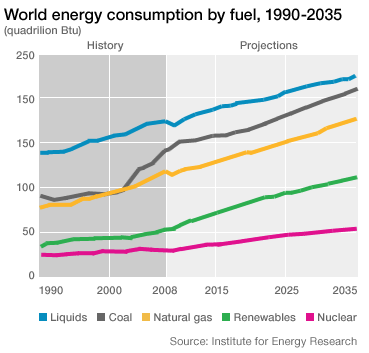
\includegraphics[width=0.33\textwidth]{test}
%      \caption{Caption}
%      \label{fig1}
%\end{figure}

Extracting resources in these ways is more expensive, and the processes are more complex. Alternatively, the industry is pursuing enhanced oil recovery from existing wells. Enhanced oil recovery takes advantage of new techniques, technology, and awareness of the geology of the field and production history to achieve higher production rates and recovery efficiency. These approaches depend on access to data. In fact, in the words of one oil and gas executive, "Drilling these days depends on data. Data collected becomes the 'eyes' guiding drilling and production."

Oil prices are experiencing greater volatility. The reasons are many, but the reality is that Brent crude prices are no longer in line with WTI crude prices. For example, in less than six months in 2012, front-month prices for Brent crude have gone from over \$120 per barrel to less than \$90 per barrel and those for WTI have gone from $110 to less than $80. The difference in price can make or break a prospect if the cost per barrel to produce comes too close to the market price. This greater volatility has oil and gas companies maintaining a constant vigil to see whether they should divest assets or continue to develop prospects.

The industry is still feeling the impact of Deepwater Horizon and San Bruno. Considerable attention is being paid to mitigating health, safety, and environment risks that come with equipment failure or operator error. In the United States, the Safety and Environmental Management System (SEMS), based on the American Petroleum Institute's RP-75, calls for owners/operators of offshore rigs to be able to identify hazards, assess environmental impact, optimize operations, develop safe work practices and training programs, and analyze incidents. The challenging physical environment in deepwater and the Arctic and the need to limit the number of personnel in hazardous and remote locations have led to the development of some fully automated rigs.

The Society of Petroleum Engineers (SPE) reports that its membership grew 12\% between 2008 and 2012, but year-over-year growth from 2007 to 2008 was 11\%. Thus, the SPE's rate of growth has slowed at a time when more engineers are needed. The implication for the oil and gas industry is that there is a need to bridge the talent gap in other ways.

The oil and gas industry is highly competitive. It used to be dominated by a few supermajors, but other competitors have emerged. In the 1970s, national oil companies controlled less than 10\% of the world's oil and gas reserves; today, they control more than 90\%. Independent exploration and production companies have made in-roads into the industry with tight oil, oil sands, and shale gas. This is not to say that there is not cooperation in the industry. Most of the deepwater projects are so expensive that they require joint development. Much of the joint development has also included national oil companies. Still there is a need in the industry to maintain competitive edge.

\section{Setting a vision for optimum smart field value}
In 2010, researchers set out to broaden their understanding of what the next 20 years could hold for the energy industry. They interviewed more than 100 high-level executives from various parts of the oil and gas ecosystem, mainly focusing
on the \emph{upstream segment}. Among the findings of \emph{Oil and
Gas 2030}: "[Executives] see integration becoming even more critical to connect the various technological disciplines and innovations with people and processes.” To them, integration is vital to delivering “the right information on demand to the right people at the right time for better decision making."

More recently, industry executives identified key barriers blocking their full realization of the benefits of smart field technologies. High on the list are the difficulties in effectively monitoring, predicting and proactively responding to oil and gas field events. Added to these is the challenge of managing a field as a total system rather than a set of isolated parts.

This helps explain why a growing number of producers are taking a different and more financially rewarding approach. Their strategy centers on fully exploiting the value of the data constantly being generated across today’s heavily instrumented oil and gas fields. Through broader consolidation and distribu- tion of this data, they are developing advanced analytical systems and other capabilities to help transform data into actionable insights serving field management and operations.

The past decade has seen the digitization of the oilfield. Whether the term is smart oil, digital oilfield, i-fields, or smart fields, in the past 10 years, digital oilfields have helped increase oilfield production. With increased digitization has come the availability of more data. According to Jay R. Pryor, vice president, business development, Chevron Corp., in a speech to the World National Oil Companies Congress 2011, "Advanced technology is the spine of 21st century energy development. Chevron's internal information technology traffic exceeds \textbf{1.5 terabytes} a day.... For example, a large seismic data processing center will gather the power of \emph{20,000 personal computers} to crunch a single seismic data set."
\\

\noindent
\textbf{High Performance Computing}\\
Processing large volumes of data is not new to the industry, however. Geologists, geophysicists, and reservoir engineers have been using massively parallel processing capabilities of high-performance computing (HPC) to perform analysis on petabytes (PB) of data to inform exploration since the late 1990s. Exploration uses sophisticated analytics such as seismic processing and reservoir modeling and simulation provided by software divisions of oilfield services companies and petrotechnical application vendors. 3D visualization is used to identify new resources. 4D visualization is also providing the ability to understand changes in a reservoir over time.

What has changed is that more sophisticated technologies are producing even more data. Starting with exploration and development, a recent innovation called wide azimuth (WAZ) is being used to increase seismic plot accuracy. WAZ involves multiple ships making multiple passes to capture a richer picture. WAZ to support exploration produces three to four times more traces per square kilometer than another acquisition technology, narrow-azimuth towed streamer (NATS). WAZ to support development has six to eight times the data volume of NATS. Onshore, Royal Dutch Shell is deploying another new technology — surface sensors developed by HP. The first test produced by the sensors created 1PB of data.

The industry has also been getting better at improving access to production data. These improvements are motivated in part by the need to more closely monitor and optimize production. Advances in telecommunications technology to access the data have also helped. Communications to remote locations have typically depended on satellite communications. However, some oil and gas companies have laid out fiber to offshore rigs — a recent investment of \$80 million for fiber in the Gulf of Mexico is an example — or stood up wireless towers to support onshore wells in remote locations.

What has also changed is the availability of new technology based on commodity hardware -- \textbf{Big Data and analytics} -- pioneered by firms such as Facebook and Google. This new technology can process high volumes of a variety of data types at relatively quicker speeds than conventional technology. Much of the new technology takes advantage of open source code such as Hadoop and MapReduce to handle large volumes of data so that the data can be processed efficiently and reliably. The ability to handle a variety of access types, including massively parallel direct access to Big Data volumes, is supported by other open source code such as Lustre.
\\

\noindent
\textbf{What\rq{}s the overall potential?}\\
Detailed modeling of an illustrative US\$2 billion mature offshore oil and gas field shows that a US\$74 million investment in smart field technology over ten years could yield \cite{IBMCAI:2011}:
\bi
\ii Total benefits: US\$326 million
\ii Payback: 37 months
\ii Ten-year ROI: 360 percent
\ei
\emph{(Note: All financial calculations are pre-tax and based on a net present value at eight percent.)}

Engineering can find it easier to manage surface and sub- surface complexity by speeding adoption of new practices
and technologies. Operations can proactively respond to critical field events. Real-time vision and revealing process insights can keep environmental teams on top of tough compliance challenges. Likewise, better monitoring and response capabilities can greatly benefit regulatory compliance. IT departments can find their own efficiencies and effective- ness through the strengths of a flexible, efficient and scalable information platform. And every improvement can bring financial benefits to help insulate the organization from price volatility and CAPEX and OPEX uncertainties.

\subsection{Mapping a practical, profitable path}
The path to smarter oil and gas field implementation consists of a series of steps that, if taken in a logical sequence, could greatly shorten time-to-value and increase investment returns. Each step supports the subsequent ones, progressing from instrumentation to integration to intelligence. Collectively, they reflect a holistic view of the field, instead of a fragmented mix of siloed technologies – as sophisticated as each may be on its own.

As Figure \ref{fig1} illustrates, the progression begins with the instrumentation of critical points in the system – ranging from surface/seafloor and wellbore data-gathering devices to real-time data feeds from drilling operations. It would also extend to safety and other facility systems, as well as export infrastructures and transport resources. The data is gathered in central repositories, where it can be analyzed, classified, formatted and labeled for future use. Meanwhile, the integrity of the various measurement and monitoring systems can be continually checked. At its heart, instrumentation can provide real-time, systemwide data users and processes can use to help them get the views and understanding of operations they need.

\begin{figure}[htb]
      \centering
      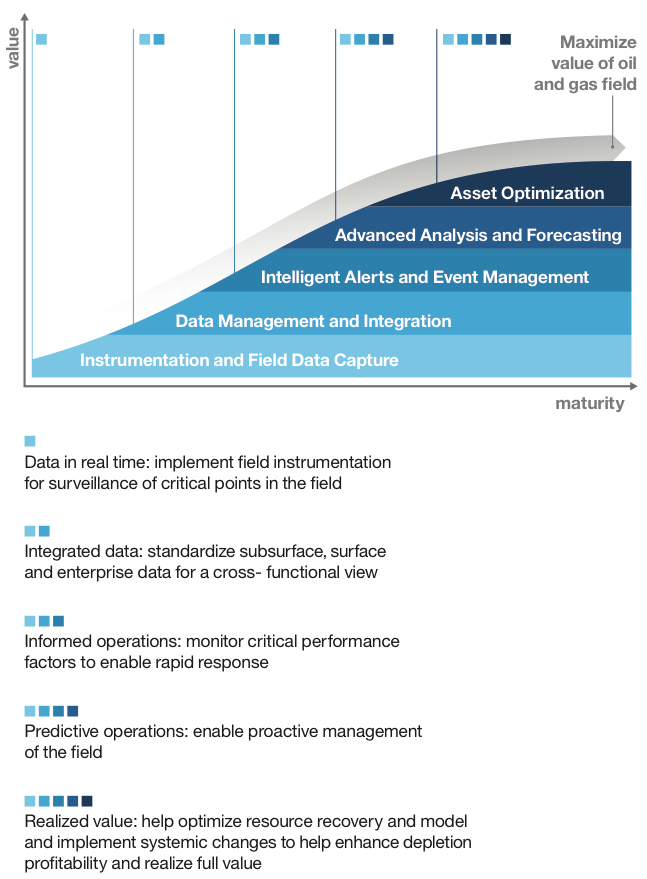
\includegraphics[width=0.4\textwidth]{figure01}
      \caption{The journey to smarter oil and gas fields.}
      \label{fig1}
\end{figure}

Each step in the progression supports those that came before, helping accelerate time-to-value and optimize returns. The steps can be applied to a particular asset, geography or organizational component, or to the entire enterprise. The key is achieving the necessary level of maturity in the preceding steps before moving on.

Though frequently overlooked or under-appreciated, the
next step is critical to the holistic management central to smart field success. Without proper integration and manage- ment of petro-technical data, organizations can severely limit the value of their installed analytical technologies. Invaluable information goes underutilized and key insights are lost.
Fortunately, where once the costs of integration could have been prohibitive, recent IT technologies have significantly lowered the cost of creating flexible, extensible infrastructures of cross-functional data. The data is set up for easy, rapid access, sharing and analysis – whether automatically by applications or by staff employing web-based, front-end portals.
Building on a strong foundation of instrumentation and integration, organizations can begin using data from multiple sources to set up intelligent alerts and event management. Alerts and alarms can be programmed to automatically trigger appropriate responses at the exact point in the field where the issue exists. Compliance management, including corrective actions and action-tracking processes, can be integrated with operational management. Workflows can be organized to better leverage the intelligent alerts. Overall, the operation can benefit from greater employee productivity, deeper under- standing of critical events, and more effective decision making.
Advanced analysis and forecasting helps move field opera- tions and management toward proactive decision making. Predictive analytics can assess and forecast the performance of wells, facilities and export systems. Models can provide insights into alternatives, along with changes in current operations and life-of-field depletion planning. Managers
can enjoy greater visibility into overall field performance – essential to more comprehensive reporting, better forecasting, faster responses and higher quality decisions and actions.


In the culminating step, the producer can reach asset optimi- zation. Information is widely shared and utilized across functions. Visualization, interactive data representation, collaboration technologies and human expertise combine. Operational management can become integrated with safety, environmental and regulatory compliance management. Workflows – operational, petro-technical and managerial – can be organized to leverage the systemwide view. Producers can benefit from better informed decisions and more effective responses reflected in everything from current operations to life-of-field depletion planning.


\lq\lq{}[BP’s] Field of the Future relies on... model-based and advanced analytical techniques to drive towards full optimization of production
and recovery for the asset or system. Applying this to wells and production optimization typically results in production uplift and staff efficiency improvements.\rq\rq{}



Leaders in the upstream petroleum industry are seeing the value of smarter oil and gas field.

For example:
\bi
\ii \textbf{Shell}: Shell reports that  \lq\lq{}Large benefits of US\$5 billion have been quantified from implementation of Smart Fields programme in some 50 Shell assets over the period of 2002 to 2009.\rq\rq{}
\ii \textbf{BP}: In 2007, Field of the Future delivered between 30 and 50 mboe/d gross production. BP plans to roll out Field
of the Future technologies to 90 percent of its production. This initiative is projected to add 1 billion barrels of oil equivalent to recovery, representing 5 percent of the current provedreservebase.
\ii \textbf{OLF}, the Norwegian Oil Industry Association, estimates that the program might generate an incremental 250 billion NOK (US\$41 billion) of NPV if implemented immediately.
\ii \textbf{Chevron}: It is hard to calculate the benefits of iField technologies, but Chevron estimates that it increases output and reduces operating costs by 2-8 percent.
\ei

\section{Breaking down the silos}
While all of the steps to the smart oil and gas field are essential, the second one – data management and integration – is worth special focus. For all the progress the industry has made in instrumentation and field data capture, integrating and fully utilizing the data remains a common and often imposing roadblock to the smart oil and gas field.
The issue is that too many petro-technical functions remain walled off from each other, making critical, real-time data inaccessible to all that could use it. And where data is being used cross-functionally, it often requires expensive manual collection, reconciliation and analysis. As E\&P magazine notes, \lq\lq{}Today, technical professionals may be spending as much as 60 percent of their time managing data\rq\rq{}”
Recognizing the impacts of the problem, many organizations have launched major process transformation initiatives to break down functional silos. They are seeking to take full advantage of instrumented, interconnected smart field technologies by focusing on three primary areas:
\bi
\ii Integrating petro-technical processes to take advantage of real-time data
\ii  Building rationalized and standardized data models
\ii  Establishing data governance and ownership processes
\ei
Technology integration is not the easiest task confronting producers, but it is essential to the success of any smart oil and gas field. Taking advantage of new, cost-efficient ways
to integrate data can make the task much less daunting. It can also open up many other opportunities for improving pro- ductivity, profitability, safety, employee retention and overall competitiveness. And the sooner it is implemented, the faster a company can see returns and the easier it will be to use new petroleum technologies to the advantage of the entire asset.


\subsection{How we put a value on \lq\lq{}smart\rq\rq{}}
The information and projections contained in this paper are based on petroleum industry research conducted by the IBM Center for Applied Insights. Case studies from 11 of the world’s leading producers were conducted to help quantify the benefits of smart oil and gas field technologies. More than a dozen executives were personally interviewed, with each interview designed to elicit clear, unbiased views of key imperatives facing the industry.
The team supplemented its primary research with data from more than 100 academic and industry studies and reports. The model for smarter upstream innovations that emerged from this research, along with the illustrative value projections, is designed to help organizations gauge the potential returns from their own, similar investments. The model can be scaled for different industry asset-types and can incorporate maturity profiles to help produce individually tailored projections that may be applicable to your organization.

\subsection{A compelling business case}
The potential value of following the path to the smart oil
and gas field becomes clearer when its financial potential is calculated. Producers can now assess how much investment would be required to \lq\lq{}smarten up\rq\rq{} virtually any field. They can then estimate what kind of return is possible from each cap- ability gained along the path. Those returns can be expressed as the combined value of four major metrics – current pro- duction, ultimate recovery, capital expense reductions and operating expense reductions.
Though each producer and each field will have different financial potential, the scale of the potential returns can be estimated and illustrated by calculating them for a represen- tative producer and field. For example, let’s estimate the returns for an illustrative organization with a fully developed field with a daily production of 20,000 barrels of oil and
20 million cubic feet of gas. Some 80 million recoverable barrels of oil equivalent are still in the ground.
Based on these and other parameters, the organization would need to invest an estimated US\$76 million to upgrade to a smart field configuration. Approximately US\$25 million of that would be spent on instrumentation and data collection.

\begin{figure}[htb]
      \centering
      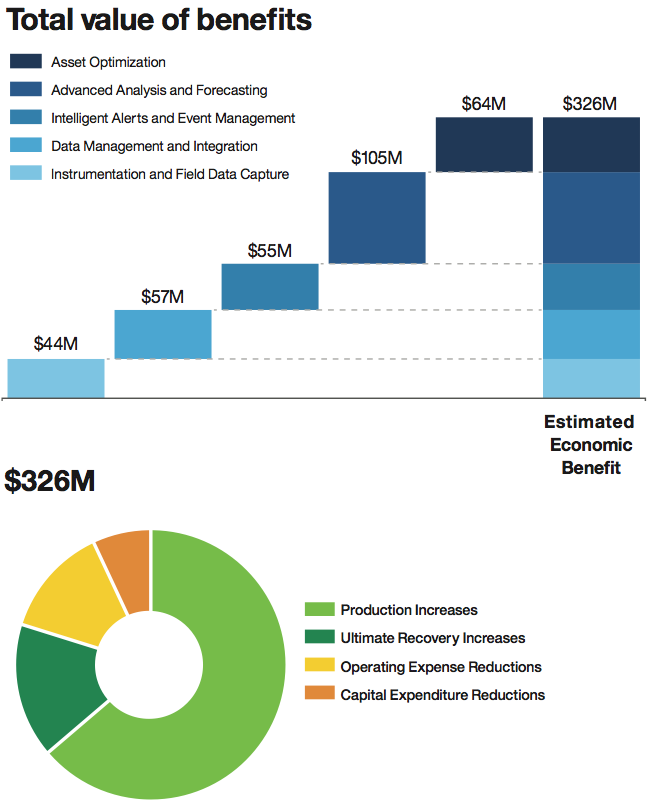
\includegraphics[width=0.4\textwidth]{figure02}
      \caption{A comprehensive implementation of smart field technologies at this illustrative field would have the potential of yielding US\$326 million on an investment of US\$76.6 million.}
      \label{fig2}
\end{figure}

\lq\lq{}\emph{...iFields will use developments in sensors, monitoring and optimization tools that anticipate and plan based on what’s happening real-time and continually adjust to operating conditions.}\rq\rq{}
–- Chevron 2006 Next Magazine



Another US\$17 million would go into building the key capability of integrating and managing the data streams from throughout the field and beyond.
Given those parameters, this producer could anticipate possible benefits on the order of US\$326 million*over ten years –
a gain of over 350 percent on that US\$76-million outlay.
Most of that value would come from new, advanced analytics – some US\$105 million. Each of the other capabilities could
also produce significant returns. And, despite the bulk of the investment occurring early on, the breakeven point could come in less than three years.

\begin{figure}[htb]
      \centering
      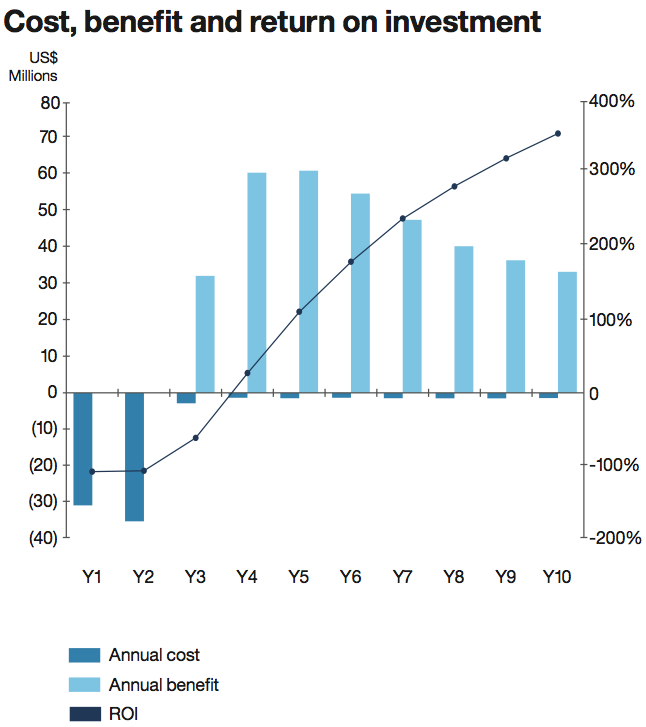
\includegraphics[width=0.4\textwidth]{figure03}
      \caption{In this illustrative case, the organization would not
need to wait long to achieve positive returns from its investment. The breakeven point would come a little past the mid-point of Year 3 and grow through the next seven years, for a cumulative projected ROI exceeding 350 percent.}
      \label{fig3}
\end{figure}

\subsection{Beyond the numbers}
The case gets even stronger when the full range of smart field benefits are considered. All are not easily quantitable but their impacts can be significant (and even more so where they overlap).

For example, a smart field’s \textbf{strategic} benefits can stem from improved planning and forecasting along with the ability to quickly respond to coming changes in the business environ- ment. Among the \textbf{operational} values are those resulting from improved safety and regulatory compliance. The organization’s \textbf{brand} can benefit as its reputation rises in parallel to its overall performance, and top talent becomes easier to recruit and retain. Meanwhile, \textbf{societal} values can accrue as the smart field helps provide a dependable and environmentally sound supply of oil and gas for an energy-dependent world.
\begin{figure}[htb]
      \centering
      
\includegraphics[width=0.4\textwidth]{figure04}
      \caption{Beyond the numbers.}
      \label{fig4}
\end{figure}

\section{Unlocking smart field benefits for your organization}
The steps described in the previous pages do not need to be undertaken on an enterprise-wide basis. One may choose to start with a particular field or even narrow it down to a single asset, geography or functional area. Investments can also
be made incrementally – beginning within a relatively short budgetary window and then spread out over multiple years.

However, it is vital to achieve a certain level of maturity at each level before moving to the next. For example, intelligent alerts are the result not only of investments in this area, but also of the instrumentation and integration put into place in the previous step.

To define the scope of your own smart field implementation projects, your organization may wish to weigh a wide range
of factors. Your overall business strategy will be an important consideration, along with a listing of your major drivers of business value. Certain imperatives may play into the decision, among them any technology adoption requirements or regulatory needs. Some organizations may want their initia- tives to enable changes in business processes and workflows.

The state and capabilities of legacy systems will be another factor – do they have inherent limitations in supplying the kind of data and control you will need? Conversely, have you developed instrumentation, field data capture capabilities and other technologies that give you a head start on reaching subsequent steps on the way to a smart field? Time devoted to answering questions like these will be well spent in terms of both accelerating and amplifying your returns from smart field development.


\section{Conclusion}
\noindent
\textbf{The growing need – and the immediate opportunity}
The years ahead will only see increasing challenges for the
oil and gas industry. As energy demand rises and easily accessed sources dwindle, petroleum organizations and the world in general can no longer afford to leave oil and gas fields under- utilized. Nor can organizations overwhelm workers with ever-increasing volumes of data without providing tools to turn that data into usable information and actionable insights.

Fortunately, there is now a suite of technologies that can
help lead the industry into a smarter future. In fact, their power and abundance make it essential for anyone evaluating a new technology to ask, “How will we avoid locking it away in a functional silo? How can we integrate the information it produces across our whole system and extract maximum value from using it?”

Answering these questions will be easier for those that have built the foundation for the smart oil and gas field. The sooner those initial steps are taken, the sooner the returns can begin. And the easier it will be to integrate new petroleum tech- nologies into the system and produce even greater value from the smart oil and gas field.









    \bibliographystyle{IEEEtran}
    \bibliography{OffshorePlant}


\end{document}
